\subsection{Relations}
\label{sec:Suggestion:Relation}

The \textsf{Relation} part provides traceability links between \textsf{MM}
elements that are \textsf{changed}, and all \viewtype elements that are 
\textsf{impacted} by that \textsf{Change}. One \textsf{MM} element
may impact several elements in the same \viewtype, but may also potentially
impact several \viewtypes. We only require so-called \emph{links}, but richer
data structures for traceability may be used \autocite{Batot-Cabot-Gerard:2021}.

The way these traceability links are computed are left as implementation
details, and may happen in two ways: \textsf{on-the-fly} imposes to create
those links every time an \textsf{MM} element is evolved; and \emph{offline}
allows for a complete evolution session to termine before triggering the
computation (based on diffing \autocite{Kehrer-Kelter-Taentzer:2011}, or using 
operation-based approaches \parencite{J:Lippe-Oosterom:1992}).
\MA{What else should be discussed here?}

\begin{figure}[t]
    \centering
    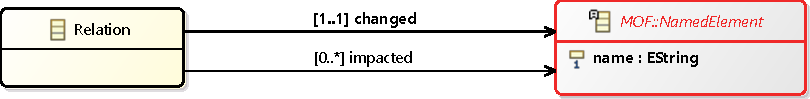
\includegraphics[width=\columnwidth]{Relation.pdf}
    \caption{Capturing \textsf{Relation}s between \textsf{MM} elements and \textsf{VT} elements.}
    \label{fig:Change}
\end{figure}